\section{Análisis de Centralidad}

\begin{figure}[H]
    \centerfloat
    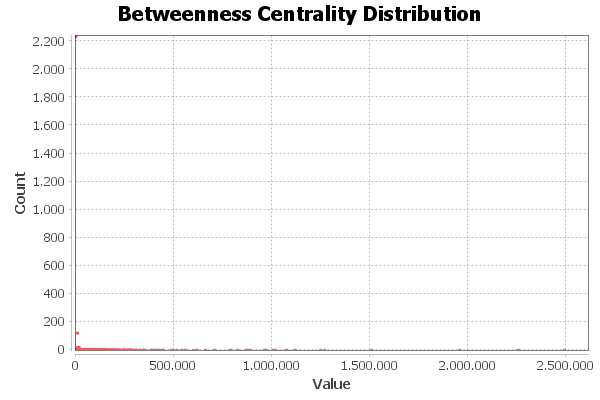
\includegraphics[width=0.9\textwidth]{img/resultados/distanciaGrafo/Betweenness Centrality Distribution.png}
    \caption{Distribución de valores de intermediación.}
\end{figure}

\begin{figure}[H]
    \centerfloat
    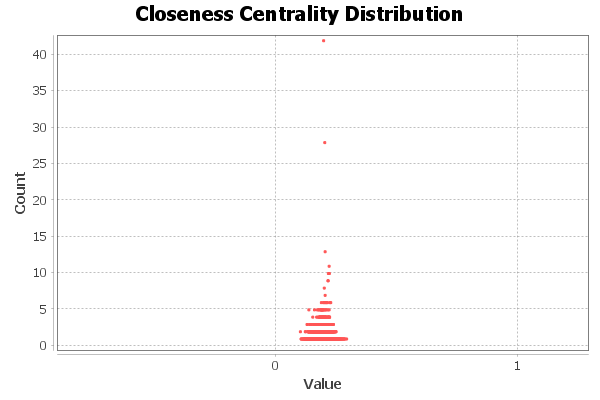
\includegraphics[width=0.9\textwidth]{img/resultados/distanciaGrafo/Closeness Centrality Distribution.png}
    \caption{Distribución de valores de cercanía.}
\end{figure}

\begin{figure}[H]
    \centerfloat
    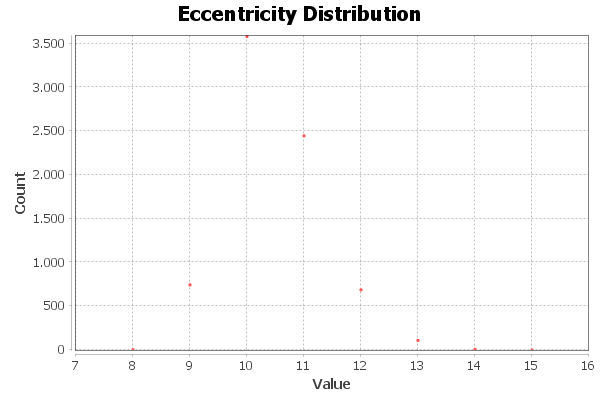
\includegraphics[width=0.9\textwidth]{img/resultados/distanciaGrafo/Eccentricity Distribution.png}
    \caption{Distribución de valores de excentricidad.}
\end{figure}

\begin{figure}[H]
    \centerfloat
    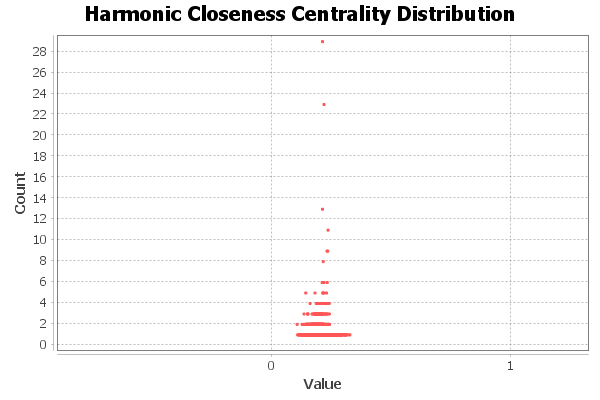
\includegraphics[width=0.9\textwidth]{img/resultados/distanciaGrafo/Harmonic Closeness Centrality Distribution.png}
    \caption{Distribución de valores de cercanía harmónica.}
\end{figure}

\begin{figure}[H]
    \centering
    \resizebox{0.9\columnwidth}{!}{%
    \begin{tabular}{| l | l | l | l |} 
        \hline
        \textbf{Centralidad de Grado} & \textbf{Intermediación} & \textbf{Cercanía} & \textbf{Vector propio} \\
        \Xhline{2\arrayrulewidth}
        \textbf{7237} - 216 & 	\textbf{7199} - 2,612,617 & \textbf{7199} - 0.2907 & 	\textbf{7237} - 1.0000  \\
        \hline
        \textbf{3530} - 175 & 	\textbf{7237} - 2,486,453 & 	\textbf{7237} - 0.2856 & \textbf{3240} - 0.7149  \\
        \hline
        \textbf{4785} - 174 & 	\textbf{2854} - 2,253,302 & 	\textbf{4356} - 0.2816 & 	\textbf{3597} - 0.7052  \\
        \hline
        \textbf{524}   - 172 & 	\textbf{4356} - 1,953,690 & 	\textbf{2854} - 0.2803 & 	\textbf{763}   - 0.6555  \\
        \hline
        \textbf{3450} - 159 & \textbf{6101} - 1,504,994 & 	\textbf{5454} - 0.2798 & 	\textbf{2083} - 0.5940  \\
        \hline
    \end{tabular}
    }
    \caption{Tabla de actores más relevantes (identificador-valor).}
\end{figure}

Respecto a la centralidad, como se comentó anteriormente estos outliers es muy probable que correspondan a creadores de contenido, ya que sus valores se encuentran extremadamente separados de la media en la red.

Acerca de la intermediación, vemos en la Figura 6 que la variación en la distribución es enorme, donde la mayoría de nodos se ubica por debajo de los 250,000. Este resultado no es extraño, el grado medio es relativamente bajo en esta red de amistad, por lo que solo un porcentaje pequeño de los nodos hacen de conexiones entre las diferentes comunidades.

\vspace{\baselineskip}

Hacemos notar que los nodos con alta intermediación tienen también los valores más altos de cercanía. No nos queda del todo claro cuál puede ser el motivo tras ello, pero es probable que estos nodos estén áltamente conectados con dos o más hubs en la red, tal y como muestra la  Figura 13.

\vspace{\baselineskip}

También nos fijamos en los valores de vector propio tras 100 iteraciones. Es de destacar una alta diferencia entre el primer actor (7237) respecto del resto, además contando con un valor de 1. Esto nos indica que la ubicación en la que se ubica en la red es muy buena, y no resulta extraño el encontrarnos enlaces con 3240, 3597 y 2083, también tres de los actores con mayor valor de vector propio.

\vspace{\baselineskip}

En las Figuras 11 y 12 se muestran los vecinos a profundidad uno y dos del nodo 7237. Vemos que ya de por sí las conexiones del actor son buenas pero además a partir de sus enlaces es capaz de extenderse a la zona más remota de la red (la inferior izquierda en la Figura 1).

\vspace{\baselineskip}

Por último, en la Figura 13 vemos la unión de los vecinos a profundidad dos del par de nodos 7237-7199. Destacamos dos cosas de esta figura: por un lado, la gran importancia de estos actores puesto que con un máximo de dos enlaces alcanzamos un 26.3\% de la red (2043 nodos); por otra, la influencia en el flujo de información ya que sabemos que \textbf{en media} añadiéndole solo cuatro enlaces más (para un total de seis) podemos transmitir a toda la red.

Estos hechos se hacen notar respectivamente en los altos valores de cercanía (una buena parte de los nodos se conectan a estos dos en pocos saltos) e intermediación (hacen de enlace entre varias comunidades). 

\begin{figure}[H]
    \centerfloat
    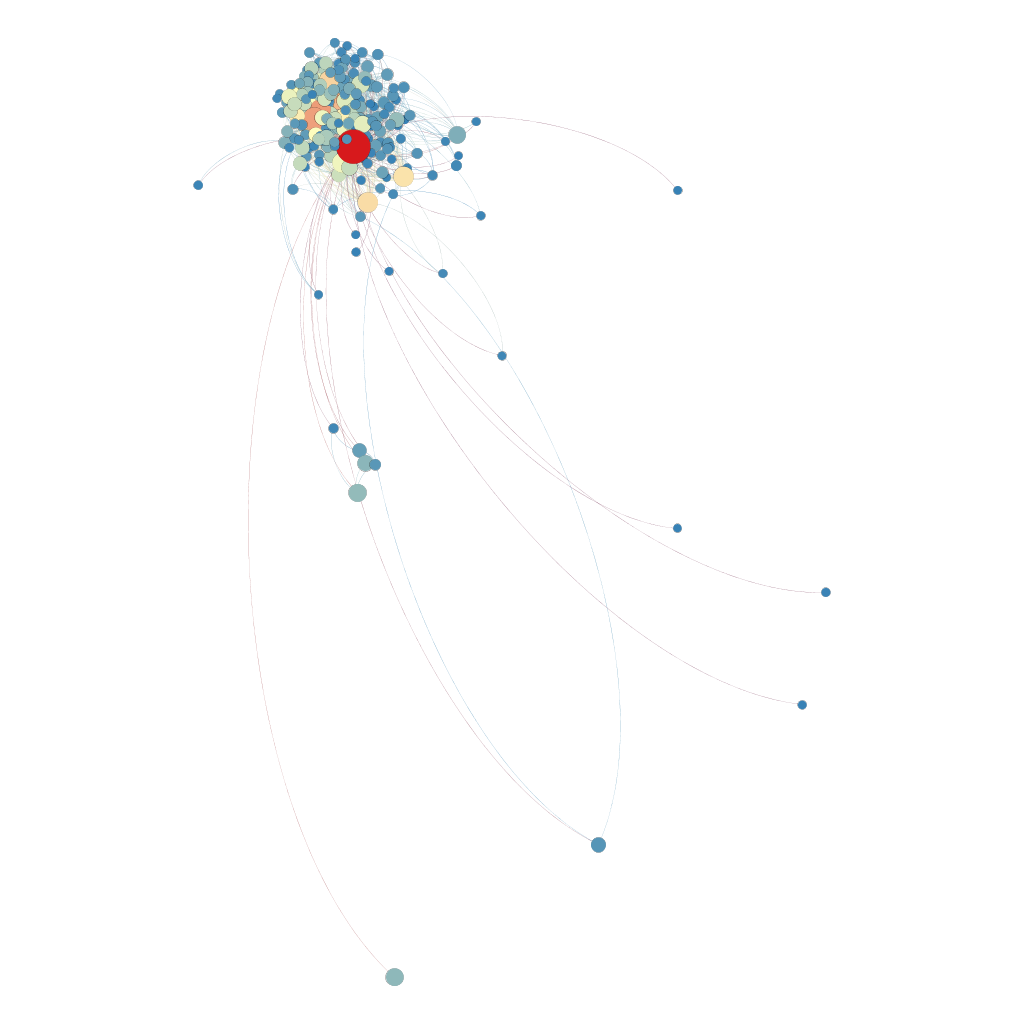
\includegraphics[width=1.3\textwidth]{img/resultados/grado-vector7237.png}
    \caption{Vecinos del nodo 7237. A mayor grado mayor tamaño, más rojo mayor valor de vector propio.}
\end{figure}

\begin{figure}[H]
    \centerfloat
    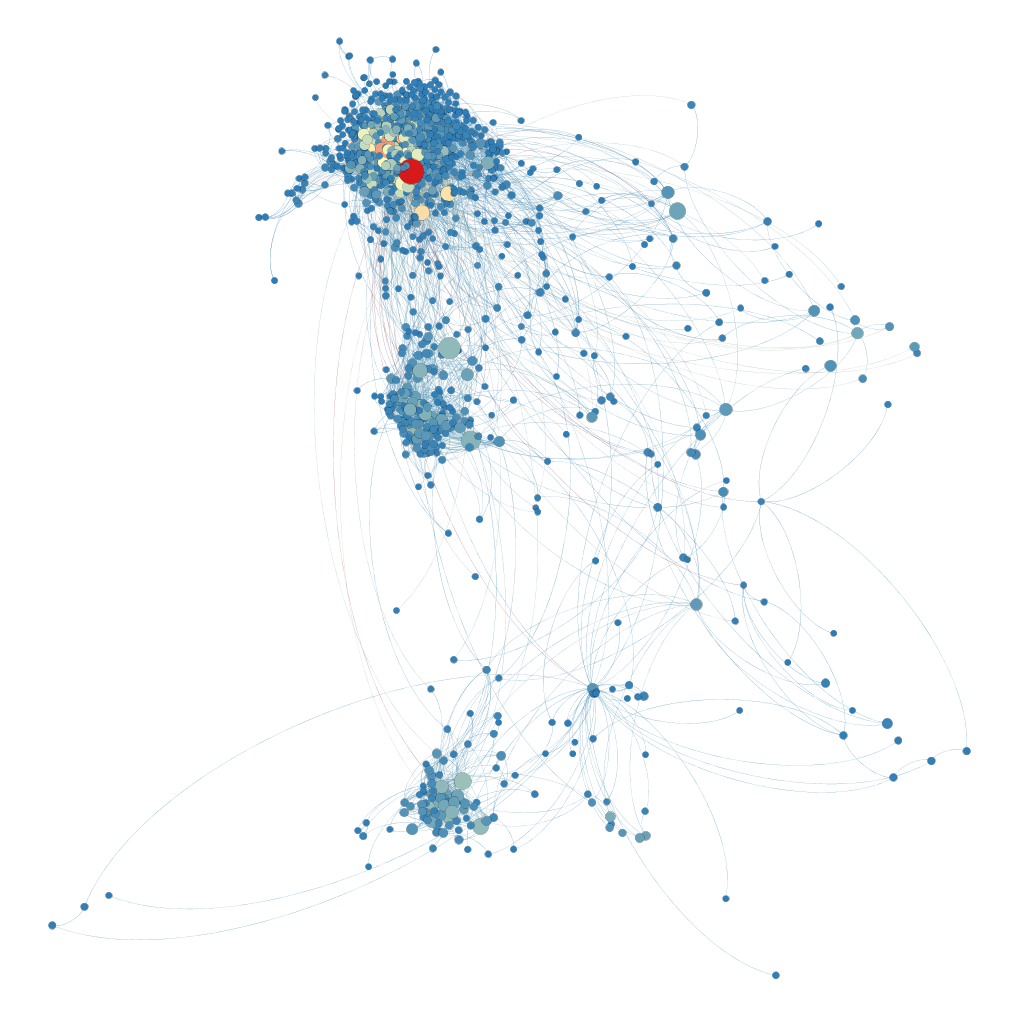
\includegraphics[width=1.3\textwidth]{img/resultados/grado-vector7237-prof2.png}
    \caption{Vecinos del nodo 7237 a profundidad 2.}
\end{figure}

\begin{figure}[H]
    \centerfloat
    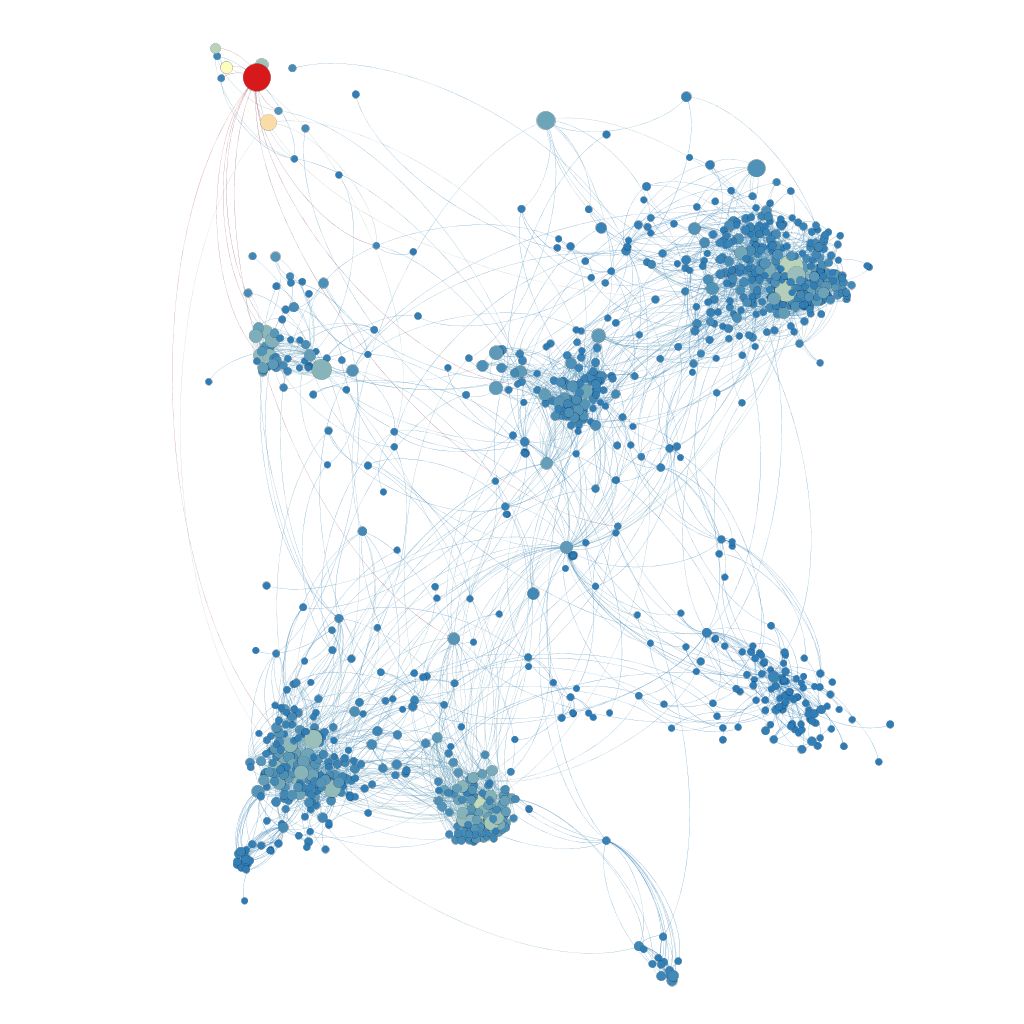
\includegraphics[width=1.3\textwidth]{img/resultados/grado-vector7199-prof2.png}
    \caption{Vecinos del nodo 7199 a profundidad 2.}
\end{figure}

\begin{figure}[H]
    \centerfloat
    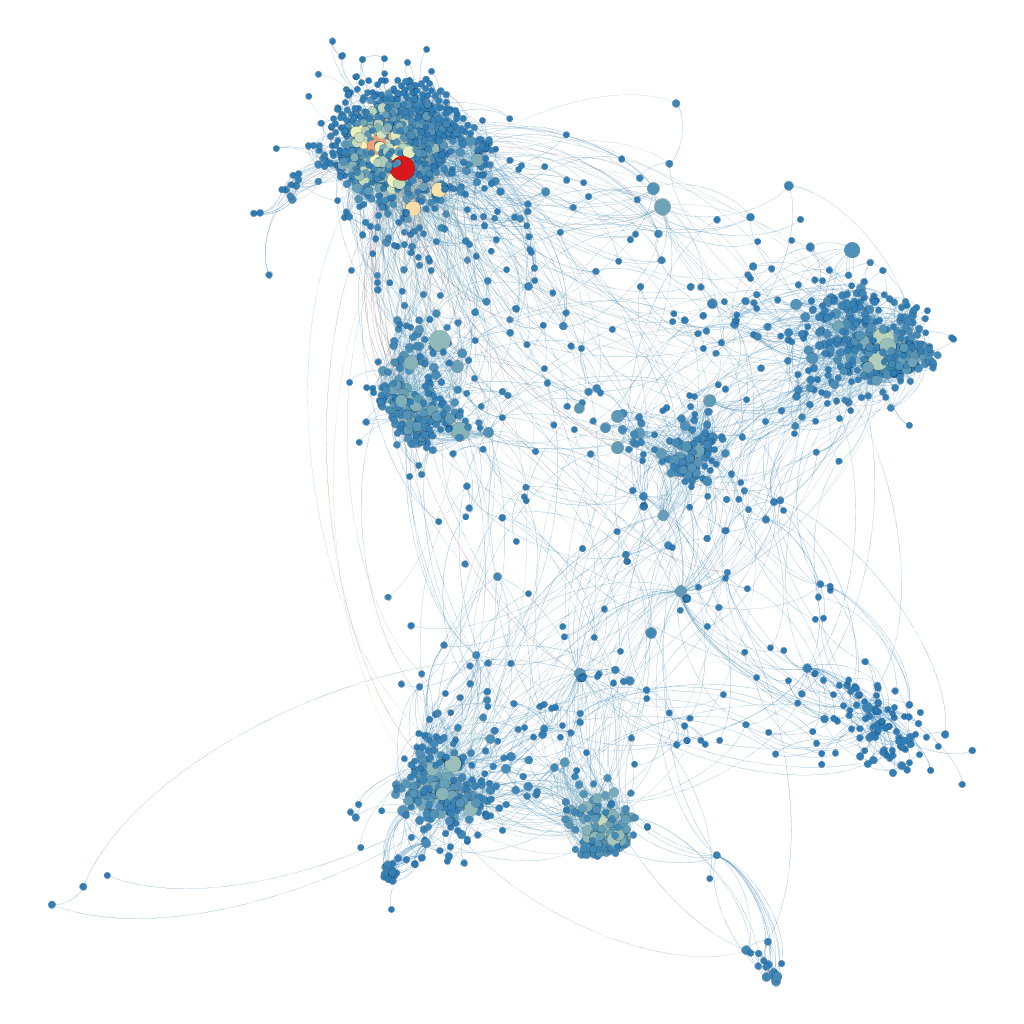
\includegraphics[width=1.3\textwidth]{img/resultados/grado-vector7199y7237.png}
    \caption{Unión de los vecinos del nodo 7237 y del 7199 a profundidad 2.}
\end{figure}